\documentclass[letterpaper]{article}
\usepackage{aaai20}
\usepackage{times}
\usepackage{helvet}
\usepackage{courier}
\usepackage[hyphens]{url} 
\usepackage{graphicx}
\graphicspath{./}
\usepackage{todonotes}
\usepackage[acronym]{glossaries}
\usepackage{enumerate}
\urlstyle{rm}
\def\UrlFont{\rm}
\usepackage{graphicx}
\frenchspacing
\setlength{\pdfpagewidth}{8.5in}
\setlength{\pdfpageheight}{11in}
\pdfinfo{
/Title (Applying CBR Retrieval and Rule-Based Heuristics to Improve Alpha-Beta Search in Chess)
/Author (Josep Han, Rowan Lavelle, Zachary Wilkerson)
}
\title{Applying CBR Retrieval and Rule-Based Heuristics to Improve Alpha-Beta Search in Chess}
\author{Josep Han, Rowan Lavelle, Zachary Wilkerson}
\date{April 2021}

\newacronym{cbr}{CBR}{case-based reasoning}

\begin{document}

\maketitle
\section{Abstract}

\begin{figure*}
    \centering
    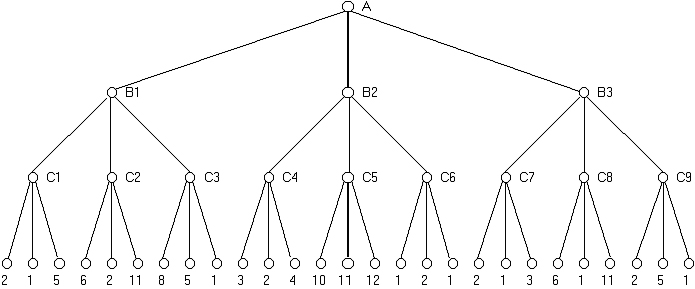
\includegraphics[width=0.65\textwidth]{minimax.jpg}
    \caption{Minimax Search Tree}
    \label{fig:my_label}
\end{figure*}

\section{Introduction}
Chess is a game almost as old as time, with the first know chess piece found in Afrasaib in Uzbekistan in 760AD. Despite a relatively simple rule set, concerning 16 pieces on a 8x8 square board where each side attempts to trap the opposing king, an incredibly complex emergent system of strategies has kept it as one of the most popular competitive board games around the world. The game has been studied for years by players of varying skill levels, from masters to novices, and chess has captured the interests of game playing AI researchers for a long time--so much so that it has been used as a metric to tell how intelligent a computer can become.

Chess is very challenging for a computer to play due to its large branching factor, which leads to an intractibly large search space.  On average there are about 32 moves a player can make at a given point, so when attempting to compute board states 4 moves ahead, there can be around $32^4=1,048,576$ possible board states, and by depth 8 $1.099 \cdot 10^{12}$ boards. As we can see this is a very large problem for computers, since most game playing AIs rely on exahustively searching deep into the search space to find good moves.

A necessary prerequisite to our research is understanding the minimax Algorithm. This is a traditional and classic game playing AI method for two player, ``zero-sum" games (i.e., one wins, and the other loses). We as humans plan our move based on what we think will be a good move, but we also consider how the opponent might respond, then we think about how we might respond to that and so on. The interesting facet here is that we are not imagining every possible move, we look at the board, see a few good moves, then employ that mental method for those moves. This is inherently very hard for computers but very simple for humans.  Minimax works the same way, however it explores \textit{everything}. It takes in a state, and then performs all possible moves, then does the same thing for each created state, up until a certain depth limit or when a terminal state is reached (win,loss,draw). When the depth limit is reached a heuristic function is called to estimate how good or bad a board is for the AI.

The algorithm then propagates the values of the heuristic back up the tree in a depth first search manner; max nodes pick the maximum value of their children, and min nodes pick the minimum values of their children. This results with a single relative best value and move being passed up the tree to the root node. An example minimax tree can be seen in Figure 1. For this tree the optimal move would be B1, since the value 5 would be propagated to the min node, and the other nodes return smaller scores.

However, this is a lot of states to visit and compute heuristic values for if the game has a large branching factor like chess. There is a classic optimization to this problem however, the alpha-beta pruning method. The method has three simple rules: if we are at a max node, we can update alpha but only increase it; if we are at a min node, we can update beta but only decrease it; and finally if at any node $\alpha \geq \beta$ then we prune, meaning we no longer consider children from that node. The intuition behind this method is that if an alpha value is propagated up to a max node, and a min node below it propagates up a beta value that is smaller, then its nonsensical to continue searching the children of that min node, since no move from that branch will ever be accepted by the above parent max node--it has already found a better move. 

This optimization of pruning is very important in chess, since it allows a deeper search in the tree through the exploration of less states. We propose methods on top of this optimization that can prune even more states, thus allowing us to explore the space faster than by just using alpha-beta pruning for game playing and board state evaluation. 

\section{Related Work}
In general, minimax and alpha-beta search are well-documented, intimately-understood topics in AI research.  At the same time, chess is a very well-studied domain for AI models, despite the apparent domination of state-of-the-art research by \textit{Deep Blue} \cite{campbell-et-al2002}, \textit{Stockfish} \cite{silver-et-al17}, \cite{grunke2020}, and \textit{AlphaZero} \cite{silver-et-al17}, \cite{grunke2020}.  Our work necessarily cannot compare directly with these models, but it is very interesting to compare and contrast approaches, as well as relative to other concepts that are not directly applied to chess.

\subsection{State-of-the-Art in Chess}
The famed \textit{Deep Blue} \cite{campbell-et-al2002} was the first chess AI to defeat a world chess champion, and it is the most similar to our work.  That said, it employed overlapping search algorithms and large databases of opening and endgame information to optimize performance (not to mention exhaustive algorithmic optimizations to minimize runtime).  In a similar vein, \textit{Stockfish} (an open-source program referenced by Silver et al. and Grünke), uses powerful search algorithms with carefully hand-crafted features to evaluate positions.  Notable among these algorithms is a so-called ``quiescence search" that modifies algorithm behavior if there is an active check or threat on the board versus a comparatively ``quiet" position; this bears some similarity to our pruning model.

In contrast to these models, \textit{AlphaZero} employs a deep neural network that is self-trained using Monte-Carlo methods to evaluate positions probabilistically \cite{silver-et-al17}.  This stands in stark contrast to the more search-oriented, rule-based algorithms discussed previously, and it offers an exciting approach that we do not consider in our research.  It is especially interesting to consider this method in the context of AI explainability, where approaches like \textit{Deep Blue} and \textit{Stockfish} are fairly readily explained, whereas the stronger \textit{AlphaZero} contains a more loosely-defined set of internal rules.  Also of interest in this vein is the less well-known \textit{DeepChess} model \cite{david-et-al2016}, which also employs neural networks to learn positional differences from the ground up.   Specifically this algorithm works in two parts, where the first part distills a provided position into a feature vector and then a second interprets the feature vector according to their training goal of evaluating positions relative to one another.

\subsection{Other Interesting Works}
Considering a final work in the realm of chess position evaluation, Kerner \cite{Kerner94} uses \acrshort{cbr} to evaluate chess positions directly, similar to the first attempt explored in the model overview section following.  Specifically, this algorithm considers key positional features (e.g., doubled pawns, material differences, etc.) as cases and then adapts them collectively to output an evaluation score for the position.  This work in particular provided inspiration for both the pruning and evaluation strategies in this research.

In terms of works not related to chess, Bradtke and Lehnert \cite{bradtke-lehnert88} propose a model using \acrshort{cbr} and search in tandem to solve puzzles.  In their approach, \acrshort{cbr} is used to place bounds on reasonable options for a search algorithm; this is different from our pruning approach but has a similar spirit.  Lastly, Anthony et al. \cite{anthony-et-al2017} explore another reinforcement learning strategy in the spirit of \textit{AlphaZero}, where their work focuses on the differentiation between planning and later generalization.  Their player outperforms state-of-the-art and professional players in the game Hex; while this work is fairly far removed from our research, it is notable in its relationship to \textit{AlphaZero}, especially for consideration of positional ideas.

\section{Model Overview}
\subsection{Heuristic Creation}
\subsubsection{Heuristic Development}The heuristic is a vital part of any AI algorithm, it allows the programmer to insert knowledge about the domain into the algorithm, thus allowing it to preform better than an uninformed algorithm.
%For chess, the heuristic or evaluation function is used to evaluate boards that appear at the max depth of the minimax search tree. The values that the heuristic returns are very integral to the AIs performance, therefore we must devise a simple yet intelligent heuristic, the trade off between complexity and run time should be balanced well.  
The heuristic we derived uses three simple but important properties of the chess board which are combined in a weighted sum to produce an overall simple, yet intelligent heuristic:

\begin{enumerate}[i]
    \item \textit{material value}: a universal score associated with each piece on the board
    \item \textit{piece positioning}: based on movement patterns, some pieces are better-placed in certain locations on the board
    \item \textit{threats}: the number of pieces we can capture versus the number of pieces of ours that are threatened
\end{enumerate}
We define the material value as a sub-heuristic considering the difference between the sum of our piece values and the sum of the opponents piece values:
$$
h_{mat} = \sum_{p \in white}\text{materialValue}(p) - \sum_{p \in black}\text{materialValue}(p)
$$
This sub-heuristic can give us a good, simple window into who is ahead in the game, based on accepted piece values defined in table \ref{materialValues}. There is no reason to define a value for the king, because if the king is missing from the board then the game is over, and that condition is already met within the minimax algorithm for the terminal states.
\begin{table}[t]
    \centering
    \begin{tabular}{|c|c|}
    \hline
        Piece & Value \\ \hline
        Pawn &  1\\ \hline
        Knight & 3\\ \hline
        Bishop & 3\\ \hline
        Rook & 5\\ \hline
        Queen & 9\\ \hline
    \end{tabular}
    \caption{Chess Piece Values}
    \label{materialValues}
\end{table}

The piece positioning sub-heuristic evaluates how well-positioned all our pieces on the board are. The values for this sub heuristic come from piece square tables (PST); a sample table for a bishop can be found in table \ref{pst}. Each piece has a unique PST that is weighted such that pieces should gradually attempt to move to certain positions with better cover, better attacking position, and more available moves. For example, pawns should attempt to advance to the end of the board, knights should attempt to stay in the middle of the board and so on. For the purpose of this sub-heuristic, we do not care about opposing piece positioning, and define the heuristic as: 
$$
h_{pos} = \sum_{p \in white}\text{PST}(p)
$$
\begin{table}[]
    \centering
    \begin{tabular}{|c|c|c|c|c|c|c|c|} \hline
        -20&-10&-10&-10&-10&-10&-10&-20\\\hline
        -10&  0&  0&  0&  0&  0&  0&-10\\\hline
        -10&  0&  5& 10& 10&  5&  0&-10\\\hline
        -10&  5&  5& 10& 10&  5&  5&-10\\\hline
        -10&  0& 10& 10& 10& 10&  0&-10\\\hline
        -10& 10& 10& 10& 10& 10& 10&-10\\\hline
        -10&  5&  0&  0&  0&  0&  5&-10\\\hline
        -20&-10&-10&-10&-10&-10&-10&-20\\\hline
    \end{tabular}
    \caption{White Bishop Piece Square Table}
    \label{pst}
\end{table}
The piece threat sub heuristic measures how many of our AI's pieces are being threatened versus how many pieces our AI is threatening. This sub-heuristic hopefully allows our AI to play more dynamic offense and defense by being sensitive to this threats-threatened ratio, and it is defined as follows:
$$
h_{threat} = \sum_{p \in black}\text{threat}(p) - \sum_{p \in white}\text{threat}(p)
$$
Where $\text{threat}(p)$ is a function that describes if $p$ is being threatened by another piece.

Thus, we can create our overall heuristic as a weighted sum of these components:
$$
H = \sum_{i} c_ih_i
$$
Where $i \in \{mat,pos,threat\}$. These weights $c_i$ can either be chosen using previous knowledge of the importance of each sub heuristic, or they can be learned.  Different weighting strategies are explored in our evaluation section.

\subsubsection{Learning Heuristic Weights}
To learn the weights $c_i$ for the heuristic, we chose to go with a genetic algorithm approach. The intuition for genetic algorithms is similar to how evolution works, in the beginning a random set of features are given to each agent, and through time (generations) and breeding (crossover and mutation) the fittest of the agents carry on, breeding better and better children and hopefully leading to a near-optimal set of parameters.

This experiment was done using ten generations of agents with five agents per generation. At the beginning, each agent was assigned a random set of weights for the heuristic, and then they played a round robin tournament (each agent plays each other agent). After the round robin was over, the three agents with the most amount of wins were selected as the fittest, these agents were then selected to breed.

Breeding works through crossover and mutation. Our crossover probability was $p=0.5$, i.e there is a 50\% chance that the child of agent A and agent B gets passed down $c_{mat}$ from agent A. this property carries over for both $c_{pos}$ and $c_{threat}$. However there is also a chance at mutation after the crossover happens, this is a vital part of evolution, given a small chance ($p=0.05$) a child has a brand new weight $c_i$ generated. This 5\% chance is applied to each of the three weights. After the 10 generations, all five winners are returned, and the top winners weights are selected to be used as the optimal heuristic weights for our pruning AI. 

\subsection{Case-Based Retrieval for Opening Play}
As of the most important parts of the chess game, the opening sequence is a heavily studied area, and any proficient player will have a few different opening sequences that they prefer to use. The opening sequences are used for general board setup before going into the mid game and generally facilitates strong piece positioning for attacking and defending.

A data set of 500 different opening sequences was found from the Encyclopedia of Chess Openings (ECO) containing around 7000 different total moves. First these moves were converted from standard algebraic notation (SAN) into string representations of the chess board by playing out each move in an opening sequence and storing the corresponding boards and moves. This became the considered case base of 500 opening sequences, along with the name of the sequence and the SAN move. Thus a case is represented as:
\begin{enumerate}[i]
    \item \textit{name}: the name of the opening sequence
    \item \textit{board}: a string representation of each board in the opening sequence
    \item \textit{move}: the SAN representation of the move used to create a given board
\end{enumerate}
Retrieving cases from the case base applied a similarity metric of Hamming distance, which is defined as:
$$
d(c_1,c_2) = \sum_{i=0}^{len(c_1)} c_{1i} \neq c_{2i}
$$
Where $c_{1i} \neq c_{2i}$ takes on the value $1$ to consider mismatched characters within the string board representation. Using this similarity metric we go through each board in each case and keep track of nearest-neighbor similarity (i.e matching to the closest board). After this, we go back through the whole case base board by board and append cases to a matched case list if they have a similarity metric to the input case that is within $2$ (not inclusive) of the minimum found distance. When returning cases, we keep track of the case name, the move index within the case at which the input case matched, and the length of the opening sequence.

At first, we only returned one case which had the maximum similarity to the input case; however this proved to be too rigid of a method, since given a board state, its not always possible to make a move that the case returns legally. To combat this, we then returned all cases that had the same maximum similarity to the input case, again this proved to be to rigid and we were not retrieving valuable cases from the case base that had good next moves. Giving the retrieval algorithm a more broad/``fuzzy" goal for case retrieval resulted in a good breadth of cases being returned, even though we are not necessarily returning only the optimal cases from a similarity standpoint. 

Once cases have been matched and returned they are sorted in decreasing order by sequence length. From the next moves following the matched cases sequence index, each move is checked for whether or not its is valid. The first valid found move is returned as the best next move for the AI to play. If no valid moves are found from the retrieved cases, the pruning AI takes over for the rest of the game.  In practice it was found that sorting the cases in decreasing order by sequence length allowed the AI to more consistently play from the same opening sequence variation. Many special variations of opening sequences are very short (3 or less moves), yet these sequences have longer more normal variations.

Finally it should be noted that when the AI is white, instead of randomly selecting an opening sequence to play, we chose to have it always play e4, and when the AI is black, if the first move is e4, it responds with c5 (the Sicilian Defense). Using previous knowledge about the game, we felt as though these were two important implementations to choose for the opening AI.

\subsection{Pruning the Search Space}
Since minimax is a search-based algorithm, it follows that a wrapper algorithm that can efficiently prune away parts of the search space from consideration potentially can improve performance.  We explore a progression of several model concepts, ultimately using a rule-based system to prune the search space using broad playing principles.

\subsubsection{1st Attempt: Case-Based Reasoning}
Intuitively, pruning away unreasonable moves from the search space appears well-suited for a \acrshort{cbr} approach, where a board state is analyzed holistically against a case base, allowing multiple specific prunings to be applied.  For example, it is traditionally unwise to move any of the pawns in front of the king after castling, as this exposes the king to attack.  In this instance, the similarity function is the location of the king (and optionally the pawns in front of it), and the solution is to prune away moves involving those pawns from consideration.  Now consider an instance where the opponent has moved their queen to a square threatened by one of the pawns.  Assuming this is not an intentional sacrifice, an exception to the case-based rule is required.  These would take the form of adaptations; continuing with the example, if a high-value piece may be captured by one of the pawns, we can override the initial solution and consider the pawn's move.  Feasibly, such a model could apply at a high resolution across diverse scenarios, including threats, pins, sacrifices, etc.

However, the granularity of this model is too fine, and the resultant cost for comparing a board state against many cases far outweighs the cost of considering the moves anyway (at least when evaluated at shallow depths like we used for testing).  Furthermore, the amount of knowledge engineering required to arrange moves in a rule-exception format is also very high.  This problem necessitates considering positional information from the board in a stricter, rule-based format that requires fewer calculations and reaches more absolute conclusions.

\subsubsection{2nd Attempt: Hierarchy of Rules}
Building on weaknesses of the \acrshort{cbr} approach, the hierarchy of rules sought define a limited set of moves to be considered by the player (pruning the rest).  This process starts with high-level situational rules that prompt specific responses.  An example situational rule might activate if a piece is threatened; specific responses might be to move the piece (especially if it is threatened by an inferior piece), to support the threatened piece with another and promote an exchange, etc.  This enables a sort of de facto pruning where moves that do not fall within the umbrella of the situational rules are pruned (e.g., if a piece is threatened, we don't care about moving some random pawn).

This strategy enjoys broad efficiency and performance advantages over the \acrshort{cbr} approach while still retaining high-resolution flexibility when a situational rule is activated.  However, this approach also fails when confronted with scenarios where most situational rules don't apply and the search space is over-pruned, leading to poor move selection.  We attempted to patch this by considering a ``catchall" situational rule, but considerations for that patch also applied when situational rules were triggered, prompting a third method instead.

\subsubsection{3rd Attempt: Combining High-Level Rules}
This final model generalizes and simplifies the rules observed in the hierarchy of rules to a simple set of four rules that are combined to generate the most performant pruning strategy observed in the project scope.  These four rules are:
\begin{enumerate}
    \item Consider moves for threatened pieces
    \item Consider moves that improve piece activity (i.e., the number of spaces they can reach/threaten)
    \item Consider moves that capture other pieces
    \item Prune moves that lead to losing exchanges
\end{enumerate}
Notably, the last of the four rules acts as a check on the other three (e.g., look for captures, but do not make captures that lead to losing exchanges), and it provides a simple framework for pruning the min player in the minimax structure.  We might be able to assume that the same pruning rules apply for both the min and max players, but a more relaxed strategy is used for the min player in case this assumption is incorrect.  While undeniably not perfect, this pruning strategy strikes a good balance between pruning aggressively but not excessively, especially in the context of the chosen heuristic.  Pruning performance against other approaches is evaluated in the following section, along with some surprising interplay with other aspects of this research.

\section{Results and Discussion}

\begin{figure*}[tb]
    \begin{center}
    \resizebox{\textwidth}{!}{
        \begin{tabular}{|c|c|c|c|c|} 
            \hline
            \multicolumn{5}{|c|}{Player 1 Per-State Runtimes}\\
            \hline
            && \multicolumn{3}{|c|}{Player 2}\\
            \hline
            Weighting & Player 1 & Base & Pruning & Human \\ [0.5ex]
            \hline\hline
            uniform & Base & - & $\mathbf{7.93*10^{-4}\pm1.46*10^{-3}}$ & $\mathit{9.90*10^{-4}\pm1.64*10^{-3}}$\\
            \hline
            base & & - & ${1.34*10^{-3}\pm2.06*10^{-3}}$ (=) & - \\
            \hline
            pruning & & - & ${1.22*10^{-3}\pm2.21*10^{-3}}$ (+)& - \\
            \hline
            handmade & & - & ${2.07*10^{-3}\pm3.59*10^{-3}}$ (+) &-\\
            \hline
            winning & & - & $\mathbf{1.31*10^{-3}\pm2.57*10^{-3}}$ &-\\
            \hline
            uniform & Pruning & $\mathbf{1.42*10^{-3}\pm2.66*10^{-3}}$ & - & $\mathit{1.45*10^{-3}\pm2.22*10^{-3}}$ \\
            \hline
            base & & ${1.19*10^{-3}\pm1.77*10^{-3}}$ (-) & - & - \\
            \hline
            pruning & & $\mathbf{1.70*10^{-3}\pm2.40*10^{-3}}$ & - & - \\
            \hline
            handmade & & ${1.35*10^{-3}\pm1.39*10^{-3}}$ (-) &- &-\\
            \hline
            winning & & ${1.32*10^{-3}\pm1.32*10^{-3}}$ (-) &- &-\\
            \hline\hline
        \end{tabular}
        }
        \resizebox{\textwidth}{!}{
        \begin{tabular}{|c|c|c|c|c|} 
            \hline
            \multicolumn{5}{|c|}{Player 2 Per-State Runtimes}\\
            \hline
            && \multicolumn{3}{|c|}{Player 1}\\
            \hline
            Weights & Player 2 & Base & Pruning & Human \\ [0.5ex]
            \hline\hline
            uniform & Base & - & $\mathit{6.89*10^{-4}\pm1.04*10^{-3}}$ &$\mathit{1.00*10^{-3}\pm1.68*10^{-3}}$\\
            \hline
            base & & - & ${8.53*10^{-4}\pm1.46*10^{-3}}$ (+) &-\\
            \hline
            pruning & & - & $\mathit{7.03*10^{-4}\pm1.13*10^{-3}}$ &-\\
            \hline
            handmade & &- & ${9.78*10^{-4}\pm1.68*10^{-3}}$ (+) &-\\
            \hline
            winning & &- & ${8.64*10^{-4}\pm1.31*10^{-3}}$ (+) &-\\
            \hline
            uniform & Pruning & $\mathit{1.30*10^{-3}\pm1.73*10^{-3}}$ & - & $\mathit{1.63*10^{-3}\pm2.25*10^{-3}}$\\
            \hline
            base & & ${1.64*10^{-3}\pm1.97*10^{-3}}$ (=) & - &-\\
            \hline
            pruning & & ${1.15*10^{-3}\pm1.11*10^{-3}}$ (-)& - &-\\
            \hline
            handmade & &${1.56*10^{-3}\pm1.72*10^{-3}}$ (-) &- &-\\
            \hline
            winning & & $\mathit{1.29*10^{-3}\pm1.62*10^{-3}}$ &- &-\\
            \hline
        \end{tabular}
        }
        \caption{Comparing per-state runtime across games, and also denoting performance.  All font styles denote the performance of the row player against the column player: bolface is a win, and italics is a loss.  For games unfinished after 150 moves (unformatted text), values include (+) for advantage, (-) for disadvantage, or (=) for equality.  Error values are one standard deviation.}
        \label{pruningEval}
    \end{center}
\end{figure*}
\subsection{Board State Evaluation}
We evaluated the performance of our algorithm by comparing the evaluation scores between our proposed Pruning Player and the algorithm without modifications, which we call Base Player.  The evaluation scores are calculated by calling the Players to recommend the best move for every move played and get the heuristic scores of the state that they calculated using the minimax algorithm. The changes in these evaluation scores are overlaid in a line graph to compare the scoring for both players (figure \ref{score_timeEval}).

Since there are different levels of play in chess games, we made sure to test games of varying levels of complexity; specifically, we picked three different chess games played by people in \url{https://lichess.org} as examples. For game selection, we used the average rating score of the players who played these games. The low level was classified when the average Elo score was in the range between 1000 and 1500; mid level was in the range 1500 to 1900, and high level in scores above 1900. We settled with games that lasted for at least 15 moves and reached a definite conclusion (i.e., no abandoned games).

Notably, as another one of the pruning algorithm’s main goals is to cut down on runtime, we also compared the cumulative time taken for each of the algorithms' evaluations (figures \ref{score_timeEval}, \ref{timeEval}).  Lastly, we set the depth factor to 4 for both algorithms in order for both algorithms to run in a reasonable amount of time.

\begin{figure*}
    \centering

    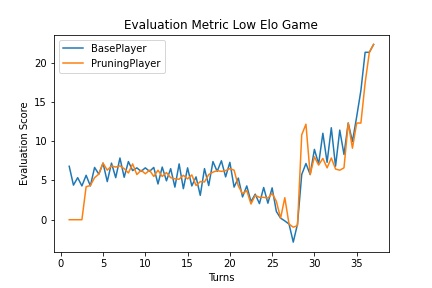
\includegraphics[scale= 0.38]{low_game_eval.jpg}
    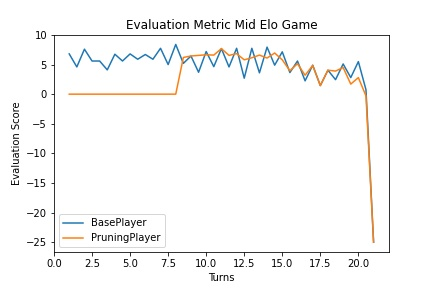
\includegraphics[scale= 0.38]{mid_game_eval.jpg}
    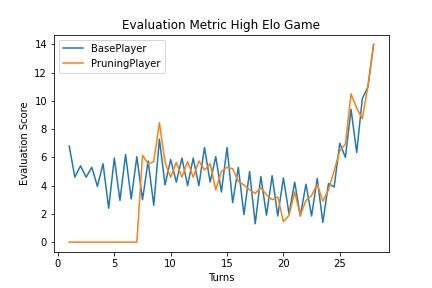
\includegraphics[scale= 0.38]{high_game_eval.jpg}

    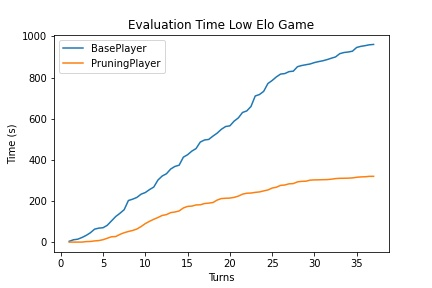
\includegraphics[scale= 0.38]{low_game_time.jpg}
    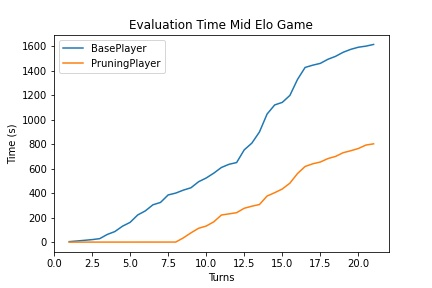
\includegraphics[scale= 0.38]{mid_game_time.jpg}
    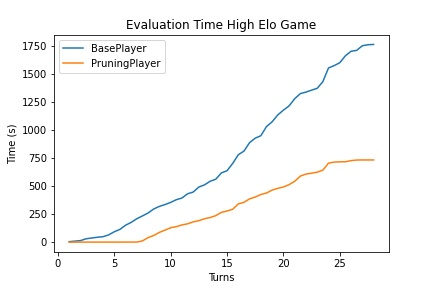
\includegraphics[scale= 0.38]{high_game_time.jpg}
  
    \caption{Comparison made between BasePlayer and PruningPlayer. Top side shows the evaluation scores determined by the Players. Note the smoother evaluation scores made by PruningPlayer on all three of the games. Bottom side shows the cumulative runtime of these Players. Note the flat lines on the Mid Elo and High Elo, indicating the Case-based retrieval at work.} 
    \label{score_timeEval}
\end{figure*}

\begin{figure}
    \center

    % 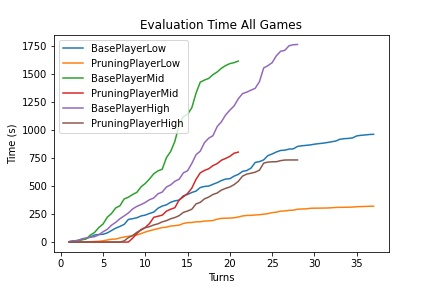
\includegraphics[width=0.48\textwidth]{all_game_time.jpg}
    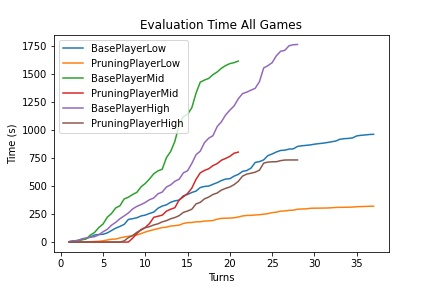
\includegraphics[scale = 0.4]{all_game_time.jpg}
    
  
    \caption{Comparison of evaluation time in all the three games.}
    \label{timeEval}
\end{figure}



\subsection{Heuristic Learning Performance}
We ran the tournament described in the methods section under three different conditions.  First, we used the base AI (which preforms no pruning) as the agent AI; for this tournament we selected any winner from the round robin as a candidate for reproduction, which was done in the hope of eliminating any very poor preforming AIs that did not win any games. Next we ran the tournament with the same setup, but using the pruning AI as our agent AI. Finally we ran a tournament using the described top three winner setup with the pruning AI as the agent AI. All three sets of weights were then put into a large round robin where we also included our knowledge chosen weights as an agent. This tournament ran for 64 games and the best heuristic weights are displayed in table \ref{weights}. It should be noted that these tournaments took a very long time to run--on average a pruning AI playing another pruning AI takes around 15 minutes. So the above described tournament played out a total of 250 games, taking around two and a half days to converge. The final round robin played out quicker in around 16 hours.

\begin{table}[t]
    \centering
    \resizebox{0.48\textwidth}{!}{
    \begin{tabular}{|c|c|c|c|} \hline
        heuristic &  material value & positioning & threats\\\hline
        weights & 9.752 &  0.111 & 3.530\\\hline
    \end{tabular}
    }
    \caption{Learned Heuristic Weights}
    \label{weights}
\end{table}

\begin{table}[]
\centering
\begin{tabular}{|l|l|l|}
\hline
 & \multicolumn{2}{l|}{Number of Moves} \\ \hline
Type & Sorted & Not Sorted \\ \hline
Pruning v. Pruning & 13.0 & 2.0 \\ \hline
Pruning v. Random & 5.8 & 5.2 \\ \hline
Pruning v. Base & 12.0 & 8.0 \\ \hline
\end{tabular}
\caption{Average Number of Moves Made by OpenAI}
\label{openings}
\end{table}

\subsection{Opening AI Performance}
Results for average number of moves played by the opening AI before switching over to the pruning AI can be seen in table \ref{openings}; this includes averages for both before and after the adaptation of sorting the cases by sequence length. Its interesting to note here that the games for Pruning versus Pruning and Pruning versus Base alpha-beta minimax are not averages, since the same game is played every time if the weights do not change.  This is due to the fact that there is no randomness within the algorithm currently. It is also interesting to note that when two pruning players play (agents who both have an opening AI component) they play out the full Sicilian Defense exchange, setting up the board very well for the rest of them game. 


\subsection{Pruning Performance}
We evaluated the pruning strategies against the Base Player through a series of head-to-head games while varying heuristic weights for each game.  The combinations considered are uniform (1.0, 1.0, 1.0), base (2.466, 0.974, 3.998; determined from the tournament of base players), pruning (2.466, 0.300, 0.120; determined from the tournament of pruning players), handmade (1, 0.02, 0.05; generated by Zach during preliminary testing), and winning (9.752, 0.111, 3.530; the best result as in table 3).  The Pruning and Base Players also play against a human player (Zach) as a comparison.  All games are played once (i.e., since the minimax algorithm is deterministic, the is no randomness in move selection), and the approaches are evaluated based on their per-state runtime and overall performance; ideally, this captures the trade-off between extra computation time and state-visiting advantages for the pruning algorithm, as well as the relative strength of the algorithms against one another (i.e., which one wins, or which one has the advantage if the game lasts longer than 150 moves).  Per-state runtime is calculated from the total time taken by minimax divided by the number of states visited less the number of dynamic programming hits.  Results are summarized in figure \ref{pruningEval}.

Notable conclusions from these data are that there are few significant differences between the Pruning Player and the Base Player.  The Base Player was generally better, but it did not dominate; the Base Player also had slightly faster average per-state computation time, but this cannot be deemed statistically significant from the Pruning Player.  It would be very interesting to consider where adding additional rules to the pruning algorithm would narrow or widen this gap.  Nonetheless, these results suggest that a pruning approach is a feasible way of injecting additional knowledge (and explanation power) into a player without significant additional cost.

So why did the Pruning Player not have a better showing?  First, since the Base Player explores all possible moves to a certain depth, the only possible improvement to be gained is if the algorithm prunes states that the heuristic would label with erroneously strong values (more on this later); generally speaking, it should not outperform a Base Player of equal strength.  On the other side of the coin, a pruning algorithm's usefulness is in speeding up calculations; this effect was not observed in our experiments (neither was a slowdown), but it is possible that the cascading effect of pruning high up in the search tree might be more strongly felt when allowing minimax to search greater depths.  Also, when combining the pruning algorithm with the opening AI, evaluation of a full game was significantly improved overall (figure \ref{score_timeEval}), which appears promising as well.

As a last point, these experiments also highlighted the sensitivity of both players to the heuristic.  Human analysis of most games finds blundered pieces for both algorithms which suggests that the both learned weights, while much better than uniform, and the heuristic itself can be further improved.  More complex heuristics would likely lead to stronger overall play and an even more interesting temporal comparison against the pruning algorithm.

\subsection{Surprising Results}
\subsubsection{Rooting out ``Red Herrings"}
Heuristics by definition cannot be perfect, and so it is possible that a reasonable move can have a similar heuristic value to an unreasonable one (especially in a weighted sum case like ours if the weights are not carefully tuned).  However, it is interesting to consider that pruning injects additional implicit information into the system, allowing for pruning of these erroneous moves with high heuristic values.  This effect is difficult to identify given our current testing structure, but future research could investigate this theory in greater detail.

\subsubsection{Opening Sensitivity}
A recurring theme of this project is finding the ``sweet spot" between efficiency and maintaining flexibility across the enormous search space that chess involves.  This appears in a novel sense in the opening phase, where the opening lookup used in our model uses thresholded \acrshort{cbr} retrieval to follow accepted opening theory.  However, the accuracy of this threshold is essential, since (as shown in some of the head-to-head tests) following an opening for too long can result in losing pieces.

\subsubsection{Evaluation Smoothing}
One of the most interesting unexpected conclusions of this project occurred in evaluation.  Notably, an evaluator using pruning broadly had a ``smoother" evaluation graph than one using only the base model.  This highlights an important consequence of minimax in chess, especially one that is significantly influenced by piece balance.  Specifically, consider a capture that occurs at the deepest point searched by minimax before applying the heuristic; the model cannot differentiate between whether the capture is sound or leads to a losing exchange.  It can only go on the material difference, which to the model is no different than if a similar piece had been captured at the root of the search tree.  This can lead to inaccurate heuristic values propagated to the top of the tree, and it also makes evaluation more extreme; this issue is alleviated by including the fourth rule described in the model section where moves leading to losing exchanges are pruned.  This makes heuristic values propagated back much more indicative of the actual material balance at that point.

\section{Conclusions and Future Work}
This research presents project work performed to investigate \acrshort{cbr}-based opening strategy, heuristic tuning, rule-based pruning, and positional evaluation in chess.  In this project, Josep Han focused on evaluation, along with detailwork and tuning of the minimax algorithm, Rowan Lavelle focused on the alpha-beta minimax algorithm, heuristic development and learning, and a case based retrieval system for opening play. Zach Wilkerson focused on pruning and object-oriented work for the minimax algorithm.  Each author presents the model and results information corresponding to their specialty section.

Although our algorithm showed promising results, we were unable to explore the full potential due to the limitation of the engine. The pruning and search algorithms are written in Python, meaning that multicore processing is not natively supported. Therefore, running evaluations and simulations took a much longer time than running the Stockfish engine, which supports multicore processing and written in C++. Consequently, increasing the evaluation depth from 4 to 5 resulted in a prohibitive amount of computation time at each turn, whereas Stockfish can utilize cores to compute at a deeper level. Adapting our code into faster engines similar to Stockfish will allow us to evaluate and simulate games at greater detail. 

\bibliographystyle{aaai}
\bibliography{references}

\end{document}
